\scanpage{31}
\margin{\figure{\begin{tikzpicture}[x=1cm,y=1cm]\draw (.12,.32)--(.1,.08)..controls(.09,.01)and(.02,.01)..(0,.05);\end{tikzpicture}}}
\margin{\figure{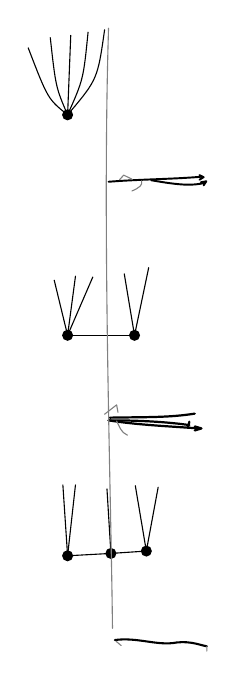
\begin{tikzpicture}[x=1cm,y=1cm,line cap=round,line join=round]
\fill (0,6.2) circle(2pt);
\draw (0,6.2)..controls(-.25,6.4)..(-.5,7.05);
\draw (0,6.2)..controls(-.15,6.55)..(-.22,7.18);
\draw (0,6.2)--(.04,7.21);
\draw (0,6.2)..controls(.2,6.65)..(.26,7.25);
\draw (0,6.2)..controls(.38,6.65)..(.47,7.28);
\draw (0,3.4)--(.85,3.4);\fill (0,3.4) circle(2pt);\fill (.85,3.4) circle(2pt);
\draw (0,3.4)--(-.17,4.1);\draw (0,3.4)--(.1,4.15);\draw (0,3.4)--(.32,4.14);
\draw (.85,3.4)--(.72,4.18);\draw (.85,3.4)--(1.03,4.26);
\draw (0,.6)--(.55,.63)--(1,.66);
\foreach \x/\y in {0/.6,.55/.63,1/.66}{\fill (\x,\y) circle(2pt);}
\draw (0,.6)--(-.06,1.5);\draw (0,.6)--(.1,1.5);\draw (.55,.63)--(.5,1.45);\draw (1,.66)--(.86,1.49);\draw (1,.66)--(1.15,1.47);
% Literal courses of the two retraced marginal arrows.
\begin{scope}[shift={(.24,5.6815)}]
\begin{scope}[x=.175cm,y=-.065cm]
\draw[line width=.7pt] (1.6,5.1)..controls (3.9,4.6) and (6.3,4.6)..(8.4,4.1);
\draw[line width=.7pt] (4.7,4.8)..controls (6.8,5.8) and (7.7,5.9)..(8.6,5.3);
\draw[gray] (2.4,4.7)--(2.7,3.8)--(3.3,4.6) (4.0,4.9)..controls (4.1,5.8) and (3.8,6.3)..(3.3,6.9);
\draw[line width=.7pt] (8.2,3.8)--(8.5,4.2)--(8.2,4.7);
\draw[line width=.7pt] (8.3,5.2)--(8.7,5.0)--(8.5,5.8);
\end{scope}
\end{scope}
\begin{scope}[shift={(.212173913,2.764637681)}]
\begin{scope}[x=.171014493cm,y=-.085507246cm]
\draw[line width=.8pt] (1.9,4.8)..controls (4.7,4.7) and (6.3,4.8)..(8.2,4.2);
\draw[line width=.8pt] (1.8,5.2)..controls (4.0,5.2) and (6.0,5.4)..(7.8,5.9);
\draw[line width=.8pt] (1.8,5.2)..controls (4.0,5.9) and (6.5,6.1)..(8.5,6.4);
\draw[gray] (1.5,4.3)--(2.4,2.9)--(2.5,4.0) (2.4,5.3)..controls (2.6,6.0) and (2.7,7.0)..(3.2,7.4);
\draw[line width=.8pt] (8.2,6.1)--(8.7,6.4)--(8.2,6.7);
\draw[line width=.8pt] (7.8,5.4)--(7.7,6.3);
\end{scope}
\end{scope}
\draw[gray] (.52,7.3)..controls(.44,4.7)and(.55,1.5)..(.57,-.32);
\begin{scope}[shift={(.328,-.0878)}]
\begin{scope}[x=.16cm,y=-.078cm]
\draw[line width=.75pt] (1.7,4.9)..controls (3.5,4.4) and (5.1,5.9)..(6.6,5.3)..controls (7.8,5.0) and (8.7,5.9)..(9.0,5.9);
\draw[gray] (1.8,5.1)--(2.2,5.8) (9.0,5.9)--(9.0,6.7);
\end{scope}
\end{scope}
\end{tikzpicture}}}


\diagram{\begin{tikzcd}[ampersand replacement=\&,column sep=9em,row sep=10em]
\begin{gathered}\mathrm{I}_{10}\ (\text{pentagonale})\\
\vcenter{\hbox{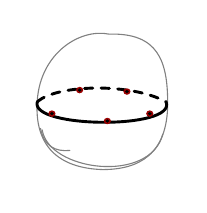
\begin{tikzpicture}[x=0.2070cm,y=-0.1870cm,line cap=round,line join=round,edge/.style={black,line width=1.05pt},rededge/.style={red!65!black,line width=.85pt},every node/.style={font=\scriptsize,inner sep=.5pt}]
\draw[gray] (1.0,5.0) .. controls (1.2,1.8) and (3.6,.1) .. (5.4,.5) .. controls (8.4,.4) and (9.0,2.3) .. (9.0,5.2) .. controls (9.0,8.7) and (7.2,9.7) .. (5.0,9.7) .. controls (2.3,9.6) and (.8,8.1) .. (1.0,5.0);
\draw[gray] (1.3,7.0) .. controls (1.7,9.8) and (7.9,10.7) .. (8.7,7.3);
\draw[gray] (1.2,6.9) .. controls (1.4,8.1) and (2.1,8.5) .. (3.0,8.4);
\draw[edge,dashed] (1.0,5.1) .. controls (2.2,3.9) and (6.8,3.8) .. (8.9,5.1);
\draw[edge] (1.0,5.1) .. controls (.5,6.9) and (9.6,7.0) .. (8.9,5.1);
\foreach \p in {(1.9,5.9),(5.3,6.4),(7.9,5.9),(3.6,4.3),(6.5,4.4)} {\fill[red!60!black] \p circle (.22);\fill[black] \p circle (.12);}
\end{tikzpicture}}}\\
\text{12 structures pentagonales sur }K\\
\{\sigma,\sigma^{-1}\}\in P_2(\mathrm{Circ}(K)\\
G\simeq\mathbb D_5\\
\widetilde G\simeq\mathbb D_5\times\{1,\sigma\}\end{gathered}\&\begin{gathered}\mathrm I_6\ (\text{bitétraédrale})\\
\vcenter{\hbox{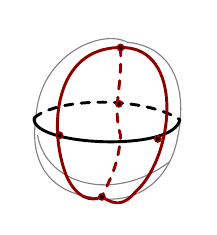
\begin{tikzpicture}[x=0.2150cm,y=-0.2230cm,line cap=round,line join=round,edge/.style={black,line width=1.05pt},rededge/.style={red!65!black,line width=.85pt},every node/.style={font=\scriptsize,inner sep=.5pt}]
\draw[gray] (1.0,5.0) .. controls (1.2,1.4) and (4.9,-.1) .. (6.4,.7) .. controls (9.6,1.0) and (10.0,4.1) .. (9.2,6.8) .. controls (8.4,9.1) and (6.4,10.0) .. (4.2,9.5) .. controls (1.8,9.2) and (.6,7.5) .. (1.0,5.0);
\draw[gray] (1.1,6.0) .. controls (1.6,8.8) and (5.6,9.9) .. (8.9,7.5);
\draw[edge,dashed] (.9,5.0) .. controls (2.4,3.8) and (7.4,3.8) .. (9.5,5.1);
\draw[edge] (.9,5.0) .. controls (.6,6.6) and (9.2,7.0) .. (9.5,5.1);
\draw[red!55!black,line width=1.05pt] (6.0,1.0) .. controls (2.1,1.0) and (1.7,5.6) .. (2.8,8.3) .. controls (3.4,9.6) and (4.3,9.8) .. (4.9,9.5);
\draw[red!55!black,line width=1.05pt] (6.0,1.0) .. controls (9.8,.9) and (9.2,7.2) .. (6.9,9.2) .. controls (6.2,10.0) and (5.7,10.0) .. (4.9,9.5);
\draw[red!55!black,line width=1.05pt,dashed] (6.0,1.0) .. controls (6.1,3.5) and (5.5,4.3) .. (6.0,6.0) .. controls (5.9,7.8) and (5.2,8.8) .. (4.9,9.5);
\foreach \p in {(6.0,1.0),(2.4,6.0),(8.2,6.2),(5.9,4.2),(4.9,9.5)} {\fill[red!60!black] \p circle (.23);\fill[black] \p circle (.12);}
\end{tikzpicture}}}\\
\text{20 structures }K=J\amalg\omega\\
\text{avec }\omega\xrightarrow{\sim}\underline\omega(J)\\
G\simeq\unsure{\mathfrak S|\mathfrak G}_J\simeq\unsure{\mathfrak S|\mathfrak G}_3\\
\widetilde G\simeq\unsure{\mathfrak S|\mathfrak G}_3\times\{1,\sigma\}\end{gathered} \arrow[r,"{3\quad f_{B,s}\quad2}","{(B\in\unsure{\mathrm{Bit\acute et}|\mathrm{Bitet}}(K),\ s\in T(B)=J)}"'] \& \begin{gathered}\mathrm I_4\ (\text{pyramidale})\\
\vcenter{\hbox{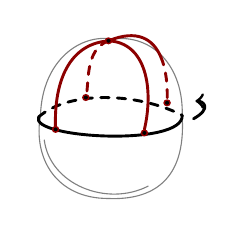
\begin{tikzpicture}[x=0.2400cm,y=-0.2250cm,line cap=round,line join=round,edge/.style={black,line width=1.05pt},rededge/.style={red!65!black,line width=.85pt},every node/.style={font=\scriptsize,inner sep=.5pt}]
\draw[gray] (.5,5.1) .. controls (.6,2.0) and (2.6,.5) .. (4.3,.8) .. controls (6.4,.5) and (8.1,2.3) .. (8.0,5.2) .. controls (8.2,8.8) and (6.4,9.9) .. (4.1,9.8) .. controls (1.3,9.8) and (.1,7.5) .. (.5,5.1);
\draw[gray] (.7,6.5) .. controls (1.0,9.0) and (4.0,10.3) .. (6.2,9.1);
\draw[edge,dashed] (.4,5.2) .. controls (2.0,3.7) and (5.6,3.8) .. (8.0,5.1);
\draw[edge] (.4,5.2) .. controls (-.1,6.4) and (8.1,6.9) .. (8.0,5.1);
\draw[red!55!black,line width=1.05pt] (4.1,.9) .. controls (1.8,1.1) and (1.2,3.6) .. (1.3,5.9);
\draw[red!55!black,line width=1.05pt] (4.1,.9) .. controls (6.1,1.0) and (6.5,3.6) .. (6.0,5.9);
\draw[red!55!black,line width=1.05pt,dashed] (4.1,.9) .. controls (2.8,1.4) and (3.1,3.4) .. (2.9,4.1);
\draw[red!55!black,line width=1.05pt] (4.1,0.9) .. controls (5.6,0.24) and (6.452,0.768) .. (6.872,1.8144);
\draw[red!55!black,line width=1.05pt,dashed] (6.872,1.8144) .. controls (7.152,2.512) and (7.24,3.44) .. (7.2,4.4);
\foreach \p in {(4.1,.9),(1.3,5.9),(6.0,6.1),(2.9,4.1),(7.2,4.4)} {\fill[red!60!black] \p circle (.20);\fill[black] \p circle (.11);}
\draw[edge,->] (8.6,5.3) .. controls (9.6,4.7) and (9.1,4.3) .. (8.7,4.3);
\end{tikzpicture}}}\\
\text{30 structures carrés orientés}\\
K=\{P\}\amalg I\\
I\ \text{structure carrée \uline{orientée}}\ (Q,\omega)=\vec Q\\
I=\coprod_{\alpha\in\delta}\alpha\qquad\delta=\text{ens. des diagonales de}\\
\omega\in\delta\wedge\bigwedge_{\alpha\in\delta}\alpha\\
G=\widetilde G=\mathbb Z/4\mathbb Z\end{gathered} \arrow[dl,bend right=10,pos=.27,"{4\quad f_{\vec Q,\omega,a}\quad2}","{(Q=\overrightarrow{\mathrm{Carr}}(K),\ a\in\Lambda(Q))}"'] \\
\begin{gathered}\mathrm{II}_2\ (\text{carré-triangle droit})\\
\vcenter{\hbox{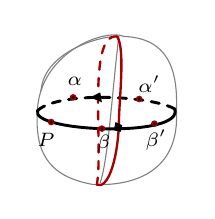
\begin{tikzpicture}[x=0.2150cm,y=-0.2090cm,line cap=round,line join=round,edge/.style={black,line width=1.05pt},rededge/.style={red!65!black,line width=.85pt},every node/.style={font=\scriptsize,inner sep=.5pt}]
\draw[gray] (.9,5.0) .. controls (1.2,1.6) and (4.9,.2) .. (6.0,.7) .. controls (8.6,.8) and (9.2,2.7) .. (9.1,5.2) .. controls (9.3,8.7) and (6.9,9.8) .. (4.2,9.7) .. controls (1.4,9.2) and (.7,7.6) .. (.9,5.0);
\draw[gray] (1.1,4.0) .. controls (1.3,1.5) and (4.9,.6) .. (5.7,.7) .. controls (5.3,4.0) and (5.1,8.0) .. (4.6,9.6);
\draw[edge,dashed] (.9,5.2) .. controls (2.2,4.0) and (7.6,4.3) .. (9.0,5.1);
\draw[edge] (.9,5.2) .. controls (.4,6.5) and (9.6,6.9) .. (9.0,5.1);
\draw[rededge] (5.6,.7) .. controls (6.1,1.5) and (5.7,4.6) .. (5.7,6.1) .. controls (5.6,8.4) and (5.0,10.0) .. (4.4,9.7);
\draw[rededge,dashed] (5.6,.7) .. controls (3.8,.5) and (4.8,7.4) .. (4.4,9.7);
\foreach \p in {(1.7,5.9),(4.7,6.3),(7.8,6.0),(3.0,4.4),(6.9,4.5)} {\fill[red!60!black] \p circle (.20);\fill[black] \p circle (.09);}
\fill (4.0,4.4)--(4.6,4.1)--(4.7,4.7)--cycle;
\fill (5.5,5.9)--(5.9,6.1)--(5.8,6.5)--(5.4,6.4)--cycle;
\node at (1.4,7.0) {$P$};\node at (4.8,7.2) {$\beta$};\node at (7.9,7.0) {$\beta'$};
\node at (3.1,3.4) {$\alpha$};\node at (7.5,3.6) {$\alpha'$};
\end{tikzpicture}}}\\
\text{2 sommets}\quad\deleted{\text{\unsure{-repères|-repère}}}\\
\text{60 structures ``pentagone}\\
\text{avec sommet'' sur }K\\
\text{i.e. }K\simeq B\amalg\omega,\ \text{avec }\omega\hookrightarrow J\\
\text{i.e. }P\in J\text{ et }\omega\simeq\omega'=B\setminus\{P\}\\
G\simeq\mathbb Z/2\mathbb Z\\
\widetilde G\simeq\mathbb Z/2\mathbb Z\times\{1,\sigma\}\end{gathered} \arrow[u,"{1\quad\gamma_{\pi,s}\quad5}","{(\pi\in\mathrm{Pent}(K),\ s\in K)}"'] \arrow[r,"{1\quad\tau_{\pi,s}=\mathrm{tw}_{1/4}\quad1}"] \& \begin{gathered}\mathrm{II}'_2=\mathrm{Tw}_{1/4}\mathrm{II}_2\\
(\text{carré-triangle gauche})\\
\text{4 sommets}\ \deleted{\text{\unsure{repères}}}\\
\vcenter{\hbox{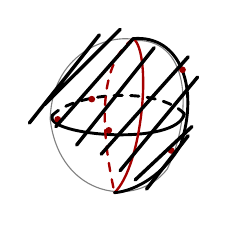
\begin{tikzpicture}[x=0.2400cm,y=-0.2330cm,line cap=round,line join=round,edge/.style={black,line width=1.05pt},rededge/.style={red!65!black,line width=.85pt},every node/.style={font=\scriptsize,inner sep=.5pt}]
% Eight explicit oblique strokes cancel this drawing; no secure alphabetic labels survive.
\draw[gray] (1.9,5.4) .. controls (2.0,1.5) and (5.4,.7) .. (6.5,1.1) .. controls (9.4,1.1) and (9.4,5.3) .. (8.1,8.1) .. controls (6.5,10.3) and (2.4,9.7) .. (1.9,5.4);
\draw[edge,dashed] (2.0,5.2) .. controls (3.2,3.9) and (7.6,3.6) .. (9.0,5.1);
\draw[edge] (2.0,5.2) .. controls (1.6,6.3) and (8.6,6.9) .. (9.0,5.1);
\draw[rededge] (6.3,1.0) .. controls (7.3,1.8) and (6.8,7.9) .. (5.3,9.4);
\draw[rededge,dashed] (6.3,1.0) .. controls (3.9,2.8) and (5.0,7.9) .. (5.3,9.4);
\draw[edge] (6.3,1.0) .. controls (8.8,.8) and (9.8,3.7) .. (8.8,6.8) .. controls (8.0,8.3) and (6.5,9.3) .. (5.3,9.4);
\foreach \p in {(2.3,5.4),(4.1,4.3),(5.0,6.0),(8.9,2.7),(8.3,7.1)} {\fill[red!60!black] \p circle (.18);}
\draw[line width=1.25pt] (.8,5.6)--(4.5,.8) (1.6,4.6)--(5.6,.5) (2.2,5.8)--(6.3,1.0) (3.3,6.8)--(7.4,1.5) (4.6,7.3)--(9.2,2.0) (5.6,8.2)--(9.7,3.1) (6.4,8.7)--(9.4,5.8) (7.0,9.2)--(9.2,6.3);
\end{tikzpicture}}}\quad\vcenter{\hbox{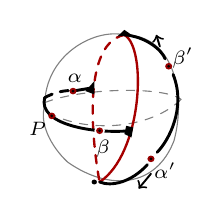
\begin{tikzpicture}[x=0.2250cm,y=-0.2100cm,line cap=round,line join=round,edge/.style={black,line width=1.05pt},rededge/.style={red!65!black,line width=.85pt},every node/.style={font=\scriptsize,inner sep=.5pt}]
\draw[gray] (1.0,4.8) .. controls (1.0,1.7) and (3.8,.1) .. (5.5,.5) .. controls (8.3,.5) and (9.0,4.1) .. (8.3,6.9) .. controls (7.3,9.7) and (4.7,10.0) .. (2.3,8.2) .. controls (1.3,7.2) and (.7,5.8) .. (1.0,4.8);
\draw[gray,dashed] (1.0,4.6) .. controls (3.1,3.7) and (7.7,3.6) .. (8.7,4.4);
\draw[gray,dashed] (1.2,5.2) .. controls (3.4,6.5) and (7.0,6.2) .. (8.7,4.4);
\draw[rededge] (5.5,.5) .. controls (6.8,1.3) and (6.5,7.7) .. (4.1,9.4);
\draw[rededge,dashed] (5.5,.5) .. controls (2.8,1.1) and (3.9,8.3) .. (4.1,9.4);
\draw[edge,dashed] (1.0,4.3) .. controls (1.5,4.0) and (2.2,3.8) .. (2.6,3.9);
\draw[edge] (1.0,4.3) .. controls (.6,5.9) and (3.7,6.5) .. (5.8,6.3);
\draw[edge] (2.6,3.9)--(3.7,3.7);
\draw[edge] (5.5,.5) .. controls (6.7,.6) and (7.6,1.4) .. (7.8,1.95);
\draw[edge] (8.25,2.9) .. controls (9.0,4.9) and (8.0,6.9) .. (7.35,7.6);
\draw[edge] (6.8,8.35) .. controls (5.9,9.4) and (4.8,9.7) .. (4.1,9.4);
\foreach \p in {(4.1,6.3)} {\fill[white] \p circle (.30);}
\foreach \p in {(1.4,5.4),(2.6,3.9),(4.1,6.3),(8.0,2.4),(7.0,8.0)} {\fill[red!60!black] \p circle (.20);\fill[black] \p circle (.09);}
\fill (3.3,3.9)--(3.8,3.3)--(3.8,4.1)--cycle;
\fill (5.6,6.0)--(6.0,6.1)--(5.9,6.7)--(5.5,6.5)--cycle;
\fill (5.1,.6)--(5.5,.2)--(5.9,.5)--cycle;\fill (3.8,9.4) circle (.15);
\draw[->,line width=.7pt] (7.5,1.2)--(7.3,.5);
\draw[->,line width=.7pt] (7.0,8.9)--(6.3,9.8);
\node at (.6,6.2) {$P$};\node at (2.7,3.1) {$\alpha$};\node at (4.3,7.4) {$\beta$};
\node at (8.8,1.9) {$\beta'$};\node at (7.8,8.7) {$\alpha'$};
\end{tikzpicture}}}\\
\text{même paramétrage que }\mathrm{II}_2\\
G\simeq\mathbb Z/2\mathbb Z,\ \widetilde G\simeq\mathbb Z/2\mathbb Z\times\{1,\sigma\}\end{gathered} \arrow[u,"{\gamma'_{\pi,s}\quad3}","{\text{comp. avec }\widetilde G;\ (\pi\in\mathrm{Pent}(K),\ s\in K)}"'] \& \begin{gathered}\mathrm{II}_1\ (\text{tétraèdre-triangle})\\
\vcenter{\hbox{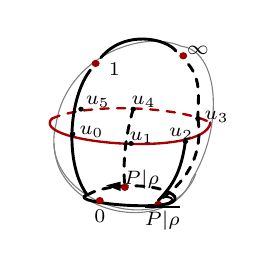
\begin{tikzpicture}[x=0.2650cm,y=-0.2420cm,line cap=round,line join=round,edge/.style={black,line width=1.05pt},rededge/.style={red!65!black,line width=.85pt},every node/.style={font=\scriptsize,inner sep=.5pt}]
\draw[gray] (.7,4.9) .. controls (1.2,1.3) and (4.9,-.1) .. (6.7,.8) .. controls (8.5,1.0) and (8.8,5.0) .. (7.2,7.8) .. controls (6.4,10.2) and (2.4,10.1) .. (1.0,7.5) .. controls (.6,6.8) and (.5,5.6) .. (.7,4.9);
\draw[gray] (.6,5.9) .. controls (.7,9.3) and (6.2,10.9) .. (7.4,7.5);
\draw[rededge,dashed] (.5,4.6) .. controls (2.3,3.7) and (6.7,4.0) .. (8.1,4.8);
\draw[rededge] (.5,4.6) .. controls (-.6,5.9) and (7.9,6.7) .. (8.1,4.8);
\draw[edge] (2.85,1.4) .. controls (4.0,-.1) and (6.0,.4) .. (6.45,1.05);
\draw[edge] (2.35,2.05) .. controls (1.3,3.5) and (1.1,7.0) .. (2.2,8.6);
\draw[edge,dashed] (7.05,1.75) .. controls (7.7,2.6) and (7.5,3.6) .. (7.5,4.6);
\draw[edge] (6.9,5.8) .. controls (6.7,7.4) and (6.3,8.1) .. (5.6,8.9);
\draw[edge,dashed] (7.5,4.6) .. controls (7.8,6.6) and (6.8,8.1) .. (5.6,8.9);
\draw[edge,dashed] (4.4,4.1) .. controls (4.0,5.6) and (3.9,7.0) .. (4.0,8.2);
\draw[edge,dashed] (2.2,8.6) .. controls (3.3,7.9) and (5.9,8.0) .. (6.4,8.7);
\draw[edge] (2.2,8.6) .. controls (1.0,9.0) and (6.8,9.6) .. (6.4,8.7);
\foreach \p in {(2.6,1.7),(6.8,1.3),(2.8,8.9),(4.0,8.2),(5.6,9.1)} {\fill[red!60!black] \p circle (.19);}
\foreach \p in {(1.5,5.4),(4.3,5.9),(6.9,5.8),(7.5,4.6),(4.4,4.1),(1.9,4.1)} {\fill \p circle (.13);}
\node at (3.5,2.0) {$1$};\node at (7.5,1.0) {$\infty$};\node at (2.8,9.7) {$0$};
\node at (4.8,7.8) {$\unsure{P|\rho}$};\node at (5.8,9.8) {$\overline{\unsure{P|\rho}}$};
\draw[line width=.7pt] (5.3,9.2)..controls (6.4,9.1) and (6.5,8.7)..(5.9,8.7);
\node at (2.4,5.3) {$u_0$};\node at (4.8,5.6) {$u_1$};\node at (6.7,5.4) {$u_2$};
\node at (8.4,4.5) {$u_3$};\node at (4.9,3.7) {$u_4$};\node at (2.7,3.7) {$u_5$};
\fill (3.1,8.1)--(3.8,7.9)--(3.8,8.4)--cycle;
\end{tikzpicture}}}\\
\text{6 sommets-repères}\\
\text{120 structures entièrement}\\
\text{épinglées,}\\
G=\deleted{\unsure{\mathbb Z_2|1}}=\{1\},\quad\widetilde G=\{1,\sigma\}\\
\left[\begin{gathered}K=J\amalg\varepsilon\quad\operatorname{card}J=3,\operatorname{card}\varepsilon=2\\\omega\in\underline\omega(J),\ r\in J\times\varepsilon\\\tau_r^0:\mathrm{II}_1(J,\varepsilon)\longrightarrow\mathrm{II}_1(u_\omega(r))\\\text{où }u_\omega=\omega\times(-1)\text{ sur }J\times\varepsilon\end{gathered}\right]\end{gathered} \arrow[ul,pos=.73,"{1\quad\gamma_r^{\unsure{0}}\quad6}","{\text{compat. avec }\widetilde G}"'] \arrow[loop right,"{\tau_r^0=\mathrm{tw}_{1/6}}"] \\
\begin{gathered}\mathrm{III}_2\ (\text{triple triangle droit})\\
\vcenter{\hbox{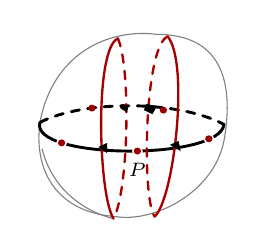
\begin{tikzpicture}[x=0.2750cm,y=-0.2600cm,line cap=round,line join=round,edge/.style={black,line width=1.05pt},rededge/.style={red!65!black,line width=.85pt},every node/.style={font=\scriptsize,inner sep=.5pt}]
\draw[gray] (.8,5.1) .. controls (1.4,1.7) and (4.0,.5) .. (6.2,.8) .. controls (9.1,.8) and (9.8,3.0) .. (9.3,6.0) .. controls (8.8,8.6) and (6.0,10.0) .. (4.3,9.7) .. controls (1.6,9.5) and (.5,7.5) .. (.8,5.1);
\draw[gray] (.9,6.4) .. controls (1.4,8.5) and (3.0,9.5) .. (4.2,9.8);
\draw[edge,dashed] (.8,5.1) .. controls (2.8,4.0) and (7.2,4.0) .. (9.3,5.2);
\draw[edge] (.8,5.1) .. controls (.3,6.9) and (9.1,7.0) .. (9.3,5.2);
\draw[rededge] (4.4,1.0) .. controls (3.3,1.5) and (3.5,8.7) .. (4.2,9.8);
\draw[rededge,dashed] (4.4,1.0) .. controls (5.0,2.4) and (4.9,8.4) .. (4.2,9.8);
\draw[rededge] (6.7,.9) .. controls (7.7,2.2) and (7.0,8.8) .. (6.1,9.7);
\draw[rededge,dashed] (6.7,.9) .. controls (5.6,1.4) and (5.5,8.9) .. (6.1,9.7);
\foreach \p in {(1.8,6.1),(5.3,6.5),(8.6,5.9)} {\fill[white] \p circle (.25);}
\foreach \p in {(1.8,6.1),(5.3,6.5),(8.6,5.9),(3.2,4.4),(6.5,4.5)} {\fill[red!60!black] \p circle (.17);}
\fill (3.5,6.3)--(3.9,6.1)--(3.9,6.6)--cycle;
\fill (6.8,6.2)--(7.2,6.0)--(7.3,6.5)--cycle;
\fill (4.6,4.2)--(4.9,4.3)--(4.8,4.6)--(4.5,4.4)--cycle;
\fill (5.7,4.2)--(6.2,4.3)--(6.0,4.7)--(5.6,4.5)--cycle;
\node at (5.3,7.4) {$P$};
\end{tikzpicture}}}\\
2+2\ \text{sommets-repère}\\
\text{60 structures ``pentagone avec}\\
\text{sommet'' sur }K,\\
G=\mathbb Z/2\mathbb Z,\widetilde G=\mathbb Z/2\mathbb Z\times\{1,\sigma\}\end{gathered} \arrow[u,start anchor=north west,"{2\quad\gamma_{\pi,\rho}\quad2}","{\begin{tikzpicture}[baseline]\draw (0,.15)..controls(-.12,.23)and(-.16,.3)..(-.14,.37);\end{tikzpicture}}"{pos=.02,description},"{(\pi\in\mathrm{Pent}(K),\rho\in\mathrm{Rep}\,\pi)}"'] \arrow[r,"{\unsure{\tau_{\pi,\omega}}}","{2\quad\tau_{\pi,\rho}=\mathrm{tw}_{1/4}\quad1}"'] \& \begin{gathered}\mathrm{III}_1\ (\text{triple triangle sem.-gauche})\\
\vcenter{\hbox{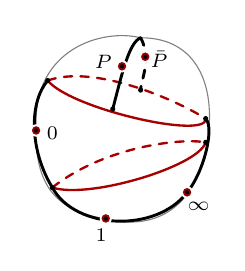
\begin{tikzpicture}[x=0.2950cm,y=-0.3020cm,line cap=round,line join=round,edge/.style={black,line width=1.05pt},rededge/.style={red!65!black,line width=.85pt},every node/.style={font=\scriptsize,inner sep=.5pt}]
\draw[gray] (1.5,5.0) .. controls (1.5,2.0) and (4.3,1.1) .. (6.0,1.5) .. controls (8.5,1.5) and (9.2,3.6) .. (8.9,5.7) .. controls (8.5,8.5) and (6.8,9.7) .. (4.4,9.1) .. controls (2.0,8.7) and (1.4,7.3) .. (1.5,5.0);
\draw[rededge,dashed] (2.0,3.3) .. controls (4.0,2.6) and (7.5,4.1) .. (8.8,4.9);
\draw[rededge] (2.0,3.3) .. controls (3.0,4.5) and (8.9,5.8) .. (8.8,4.9);
\draw[rededge,dashed] (2.2,7.8) .. controls (4.4,6.1) and (7.7,5.7) .. (8.8,5.9);
\draw[rededge] (2.2,7.8) .. controls (3.8,8.3) and (8.5,6.9) .. (8.8,5.9);
\draw[edge] (2.0,3.3) .. controls (1.2,4.2) and (1.2,6.2) .. (2.2,7.8) .. controls (3.2,9.6) and (6.7,9.7) .. (8.0,8.0) .. controls (8.7,7.2) and (9.2,5.3) .. (8.8,4.9);
\draw[edge] (4.8,4.5) .. controls (5.2,3.0) and (5.5,1.7) .. (6.0,1.5);
\draw[edge,dashed] (6.0,1.5) .. controls (6.5,2.4) and (6.0,3.3) .. (6.0,3.7);
\foreach \p in {(1.5,5.4),(4.5,9.1),(8.0,8.0),(5.2,2.7),(6.2,2.3)} {\fill[white] \p circle (.26);}
\foreach \p in {(1.5,5.4),(4.5,9.1),(8.0,8.0),(5.2,2.7),(6.2,2.3)} {\fill[red!60!black] \p circle (.18);\fill[black] \p circle (.09);}
\foreach \p in {(2.0,3.3),(4.8,4.5),(6.0,3.7),(8.8,4.9),(8.8,5.9),(2.2,7.8)} {\fill \p circle (.11);}
\node at (2.2,5.5) {$0$};\node at (4.3,9.8) {$1$};\node at (8.5,8.6) {$\infty$};
\node at (4.4,2.5) {$P$};\node at (6.8,2.4) {$\bar P$};
\end{tikzpicture}}}\quad=\quad\vcenter{\hbox{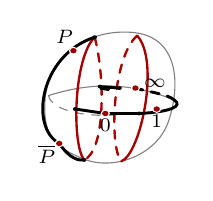
\begin{tikzpicture}[x=0.2250cm,y=-0.1900cm,line cap=round,line join=round,edge/.style={black,line width=1.05pt},rededge/.style={red!65!black,line width=.85pt},every node/.style={font=\scriptsize,inner sep=.5pt}]
\draw[gray] (1.7,5.0) .. controls (2.0,1.5) and (4.7,.3) .. (6.8,.6) .. controls (9.3,1.0) and (9.3,4.2) .. (8.7,6.4) .. controls (8.1,8.8) and (5.5,9.9) .. (3.8,9.0) .. controls (1.9,8.1) and (1.6,7.1) .. (1.7,5.0);
\draw[gray] (1.9,4.8) .. controls (4.3,3.9) and (6.5,3.9) .. (9.0,5.1);
\draw[gray,dashed] (1.9,4.8) .. controls (2.0,5.8) and (4.3,6.5) .. (6.9,5.9);
\draw[rededge] (4.5,.9) .. controls (3.3,2.3) and (3.2,8.0) .. (3.9,9.1);
\draw[rededge,dashed] (4.5,.9) .. controls (5.1,3.6) and (5.1,8.5) .. (3.9,9.1);
\draw[rededge] (6.9,.8) .. controls (8.2,2.5) and (7.1,8.7) .. (6.0,9.2);
\draw[rededge,dashed] (6.9,.8) .. controls (5.5,2.2) and (5.3,8.2) .. (6.0,9.2);
\draw[edge] (4.5,.9) .. controls (1.4,2.1) and (.8,6.9) .. (2.5,8.0) .. controls (2.9,8.7) and (3.4,9.2) .. (3.9,9.1);
\draw[edge] (3.4,5.7)--(5.1,6.0)--(7.0,6.0) .. controls (8.8,5.9) and (9.5,5.5) .. (9.0,5.1);
\draw[edge,dashed] (9.0,5.1) .. controls (8.6,4.7) and (7.7,4.6) .. (6.8,4.3);
\draw[edge] (4.8,4.2)--(5.9,4.3);
\foreach \p in {(3.3,1.8),(2.5,8.0),(5.1,6.0),(8.0,5.7),(6.8,4.3)} {\fill[white] \p circle (.26);}
\foreach \p in {(3.3,1.8),(2.5,8.0),(5.1,6.0),(8.0,5.7),(6.8,4.3)} {\fill[red!60!black] \p circle (.18);}
\foreach \p in {(4.5,.9),(3.4,5.7),(3.9,9.1),(7.0,6.0),(4.8,4.2),(5.9,4.3)} {\fill \p circle (.13);}
\fill (4.8,4.1)--(5.4,4.3)--(5.3,4.5)--(4.8,4.4)--cycle;
\node at (2.8,.9) {$P$};\node at (1.8,8.7) {$\overline P$};\node at (5.1,6.8) {$0$};\node at (8.0,6.5) {$1$};\node at (7.9,4.0) {$\infty$};
\end{tikzpicture}}}\\
\text{2+4 sommets-repère}\\
\text{120 structures épinglées}\\
G=1,\widetilde G=\{1,\sigma\}\end{gathered} \arrow[u,"{1\quad\gamma_r^1\quad2}"] \arrow[ur,"{3\qquad3}","{(r\in\mathrm{Rep}(K))}"',"{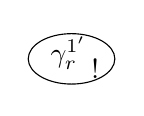
\begin{tikzpicture}[baseline=-.6ex]\draw (0,0) ellipse (.55 and .32);\node at (-.04,.07) {$\gamma_r^{1'}$};\node at (.3,-.13) {$!$};\end{tikzpicture}}"{description}] \arrow[r,"{1\quad\tau'_r\quad2}"] \& \begin{gathered}\mathrm{III}'_2\ (\text{triple triangle gauche})\\
\vcenter{\hbox{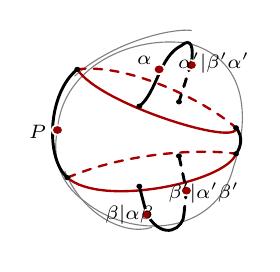
\begin{tikzpicture}[x=0.3150cm,y=-0.2750cm,line cap=round,line join=round,edge/.style={black,line width=1.05pt},rededge/.style={red!65!black,line width=.85pt},every node/.style={font=\scriptsize,inner sep=.5pt}]
\draw[gray] (1.5,5.0) .. controls (1.7,2.0) and (4.6,.6) .. (6.8,1.0) .. controls (9.3,1.8) and (9.2,4.7) .. (8.6,6.7) .. controls (7.9,9.9) and (4.5,10.1) .. (2.6,8.3) .. controls (1.5,7.4) and (1.3,6.1) .. (1.5,5.0);
\draw[gray] (2.2,2.5) .. controls (3.8,.9) and (6.1,.3) .. (6.9,.4);
\draw[gray] (1.8,6.9) .. controls (2.5,8.9) and (4.2,9.9) .. (5.3,9.5);
\draw[rededge,dashed] (2.3,2.2) .. controls (4.3,1.9) and (7.4,3.6) .. (8.7,4.9);
\draw[rededge] (2.3,2.2) .. controls (3.2,3.8) and (8.8,5.8) .. (8.7,4.9);
\draw[rededge,dashed] (1.9,7.2) .. controls (4.6,5.9) and (7.7,5.9) .. (8.7,6.1);
\draw[rededge] (1.9,7.2) .. controls (3.3,8.6) and (8.3,7.4) .. (8.7,6.1);
\draw[edge] (2.3,2.2) .. controls (1.1,3.3) and (1.0,6.3) .. (1.9,7.2);
\draw[edge] (8.7,4.9) .. controls (9.0,5.3) and (8.9,5.8) .. (8.7,6.1);
\draw[edge] (4.8,3.9) .. controls (5.5,3.3) and (5.6,1.6) .. (6.5,1.1) .. controls (6.9,.7) and (7.0,1.2) .. (6.9,1.9);
\draw[edge,dashed] (6.9,1.9)--(6.4,3.7);
\draw[edge] (4.8,7.6)--(5.1,8.9) .. controls (5.8,10.2) and (6.6,9.5) .. (6.6,8.9);
\draw[edge,dashed] (6.6,8.9)--(6.7,7.8)--(6.4,6.2);
\foreach \p in {(1.5,5.0),(5.6,2.2),(6.9,2.0),(5.1,8.9),(6.7,7.8)} {\fill[white] \p circle (.26);}
\foreach \p in {(1.5,5.0),(5.6,2.2),(6.9,2.0),(5.1,8.9),(6.7,7.8)} {\fill[red!60!black] \p circle (.18);}
\foreach \p in {(2.3,2.2),(4.8,3.9),(6.4,3.7),(8.7,4.9),(8.7,6.1),(6.4,6.2),(4.8,7.6),(1.9,7.2)} {\fill \p circle (.12);}
\node at (.7,5.1) {$P$};\node at (5.0,1.8) {$\alpha$};
\node at (7.8,1.9) {$\unsure{\alpha'|\deleted{\beta'}\inserted{\alpha'}}$};
\node at (4.4,8.9) {$\unsure{\beta|\deleted{\alpha}\inserted{\beta}}$};
\node at (7.4,7.9) {$\unsure{\beta'|\deleted{\alpha'}\inserted{\beta'}}$};
\end{tikzpicture}}}\quad\simeq\quad\vcenter{\hbox{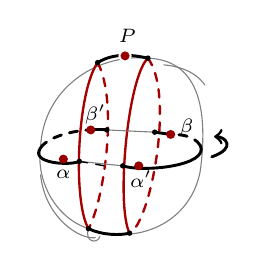
\begin{tikzpicture}[x=0.2900cm,y=-0.2850cm,line cap=round,line join=round,edge/.style={black,line width=1.05pt},rededge/.style={red!65!black,line width=.85pt},every node/.style={font=\scriptsize,inner sep=.5pt}]
\draw[gray] (.7,5.4) .. controls (.8,2.8) and (3.1,1.2) .. (5.4,1.4) .. controls (7.8,1.5) and (8.0,4.0) .. (7.7,6.4) .. controls (7.3,8.7) and (5.0,9.8) .. (2.8,9.0) .. controls (1.3,8.5) and (.5,6.8) .. (.7,5.4);
\draw[gray] (.7,6.6) .. controls (.9,8.5) and (2.4,9.5) .. (3.1,9.4);
\draw[gray] (6.1,1.7) .. controls (7.2,1.8) and (7.7,2.3) .. (7.9,2.6);
\draw[rededge] (3.2,1.6) .. controls (2.3,2.9) and (2.1,7.8) .. (2.8,9.0);
\draw[rededge,dashed] (3.2,1.6) .. controls (4.1,3.3) and (3.5,7.7) .. (2.8,9.0);
\draw[rededge] (5.4,1.4) .. controls (4.5,2.3) and (4.0,8.0) .. (4.6,9.2);
\draw[rededge,dashed] (5.4,1.4) .. controls (6.6,3.0) and (5.5,8.8) .. (4.6,9.2);
\draw[edge] (3.2,1.6) .. controls (4.0,1.1) and (4.9,1.3) .. (5.4,1.4);
\draw[edge] (2.8,9.0) .. controls (3.4,9.3) and (4.2,9.3) .. (4.6,9.2);
\draw[gray] (2.4,6.0)--(4.3,6.2);
\draw[gray] (3.6,4.6)--(5.7,4.7);
\draw[edge,dashed] (.7,5.4) .. controls (1.1,4.8) and (2.6,4.5) .. (3.6,4.6);
\draw[edge] (.7,5.4) .. controls (.2,6.1) and (2.0,6.2) .. (2.4,6.0);
\draw[line width=.5pt,dashed] (2.4,6.0)--(3.5,6.2);
\draw[edge] (4.3,6.2) .. controls (5.2,6.5) and (8.1,6.2) .. (7.7,5.3);
\draw[edge,dashed] (7.7,5.3) .. controls (7.4,4.8) and (6.7,4.8) .. (6.4,4.8);
\draw[edge] (6.4,4.8)--(5.7,4.7);
\draw[edge] (2.9,4.6)--(3.6,4.6);
\draw[gray] (2.8,9.0)..controls(2.6,9.6)and(3.2,9.7)..(3.3,9.35);
\foreach \p in {(4.4,1.3)} {\fill[white] \p circle (.29);}
\foreach \p in {(4.4,1.3),(1.7,5.9),(5.0,6.2),(2.9,4.6),(6.4,4.8)} {\fill[red!60!black] \p circle (.20);}
\foreach \p in {(3.2,1.6),(5.4,1.4),(2.8,9.0),(4.6,9.2),(2.4,6.0),(4.3,6.2),(3.6,4.6),(5.7,4.7)} {\fill \p circle (.12);}
\node at (4.5,.4) {$P$};\node at (1.7,6.6) {$\alpha$};\node at (5.1,6.8) {$\alpha'$};\node at (3.1,3.9) {$\beta'$};\node at (7.1,4.5) {$\beta$};
\draw[edge,->] (8.2,5.8) .. controls (9.3,5.4) and (8.8,4.9) .. (8.3,4.9);
\end{tikzpicture}}}\\
\text{4+4 sommets-repère}\\
\text{60 structures de carré orienté à}\\
\text{\unsure{codiagonales|codiagonale}, }K=\{P\}\amalg I,\\
I\ \text{muni d’une \inserted{str.} \unsure{carré|carrée} en \unsure{codiagonales|codiagonale} }\delta=\{\{\alpha,\beta\},\{\alpha',\beta'\}\}\\
\text{i.e. d’un repère de }\unsure{\mathfrak X|\mathbb J}\unsure{(}I)\\
G=\mathbb Z/2\mathbb Z\unsure{\deleted{*}},\quad\widetilde G\simeq\mathbb Z/2\mathbb Z\times\mathbb Z/2\mathbb Z\simeq\mathbb Z/2\mathbb Z\times\{1,\sigma\}\end{gathered} \arrow[uu,bend right=70,"{1\quad\gamma_r^{2'}\quad2}"] \arrow[ull,bend left=65,"{2\quad\gamma_r^2\quad2}"']
\end{tikzcd}}
% crop-candidate: scan 31

\diagram{\[\begin{array}{lll}
\uline{\text{niveau }2}&\mathrm I_{10},\mathrm I_6,\mathrm I_4&12+20+30=62\\
\uline{\text{niveau }}1&\mathrm{II}_2,\mathrm{II}'_2,\mathrm{II}_1&60+60+120=240\\
\uline{\text{niveau }}0&\mathrm{III}_2,\mathrm{III}_4,\mathrm{III}'_2&60+120+60=240\\
&&\overline{542}
\end{array}\]}

(l’indice ``i'' indique l’ordre du \(G=\operatorname{Aut}^{+}\unsure{\}|)}\), donc le nb de structures \deleted{est} \(120/i\))

\uline{NB} Sauf \(\mathrm I_4\), toutes ces structures sont ``réelles''.

\[\begin{array}{ll}
\pi\in\mathrm{Pent}(K),&B\in\mathrm{Bit\acute et}(K)\\
s\in K,&\vec Q\in\overrightarrow{\mathrm{Carr}}(K)\\
\rho\in\mathrm{Rep}(\pi);&r\in\mathrm{Rep}(K)
\end{array}\]
(\uline{NB} \(\{(\pi,\rho)\}\unsure{\simeq}\mathrm{Rep}(K)\)).
\margin{30}
